%%%% Paramétrage du TD %%%%
\def\xxactivite{Activation 1 \ifprof -- Corrigé \else \fi} % \normalsize \vspace{-.4cm}
\def\xxauteur{\textsl{Xavier Pessoles}}


\def\xxnumchapitre{Chapitre 1 \vspace{.2cm}}
\def\xxchapitre{\hspace{.12cm} Correction des systèmes}


\def\xxcompetences{%
\vspace{-.3cm}
\textsl{%
\textbf{Savoirs et compétences :}\\
\vspace{-.4cm}
%\begin{itemize}[label=\ding{112},font=\color{ocre}] 
%\item \textit{Res1.C4 : } Correction
%\item \textit{Con.C2.SF1 : } Choisir un type de correcteur adapté
%\end{itemize}
}}

\def\xxtitreexo{Activation -- Système de dépose de composants électroniques}%Motorisation du moteur Haibike}
\def\xxsourceexo{\hspace{.2cm} \footnotesize{Émilien Durif -- E3A PSI 2011}}
%\def\xxauteur{\textsl{Xavier Pessoles}}

\def\xxfigures{
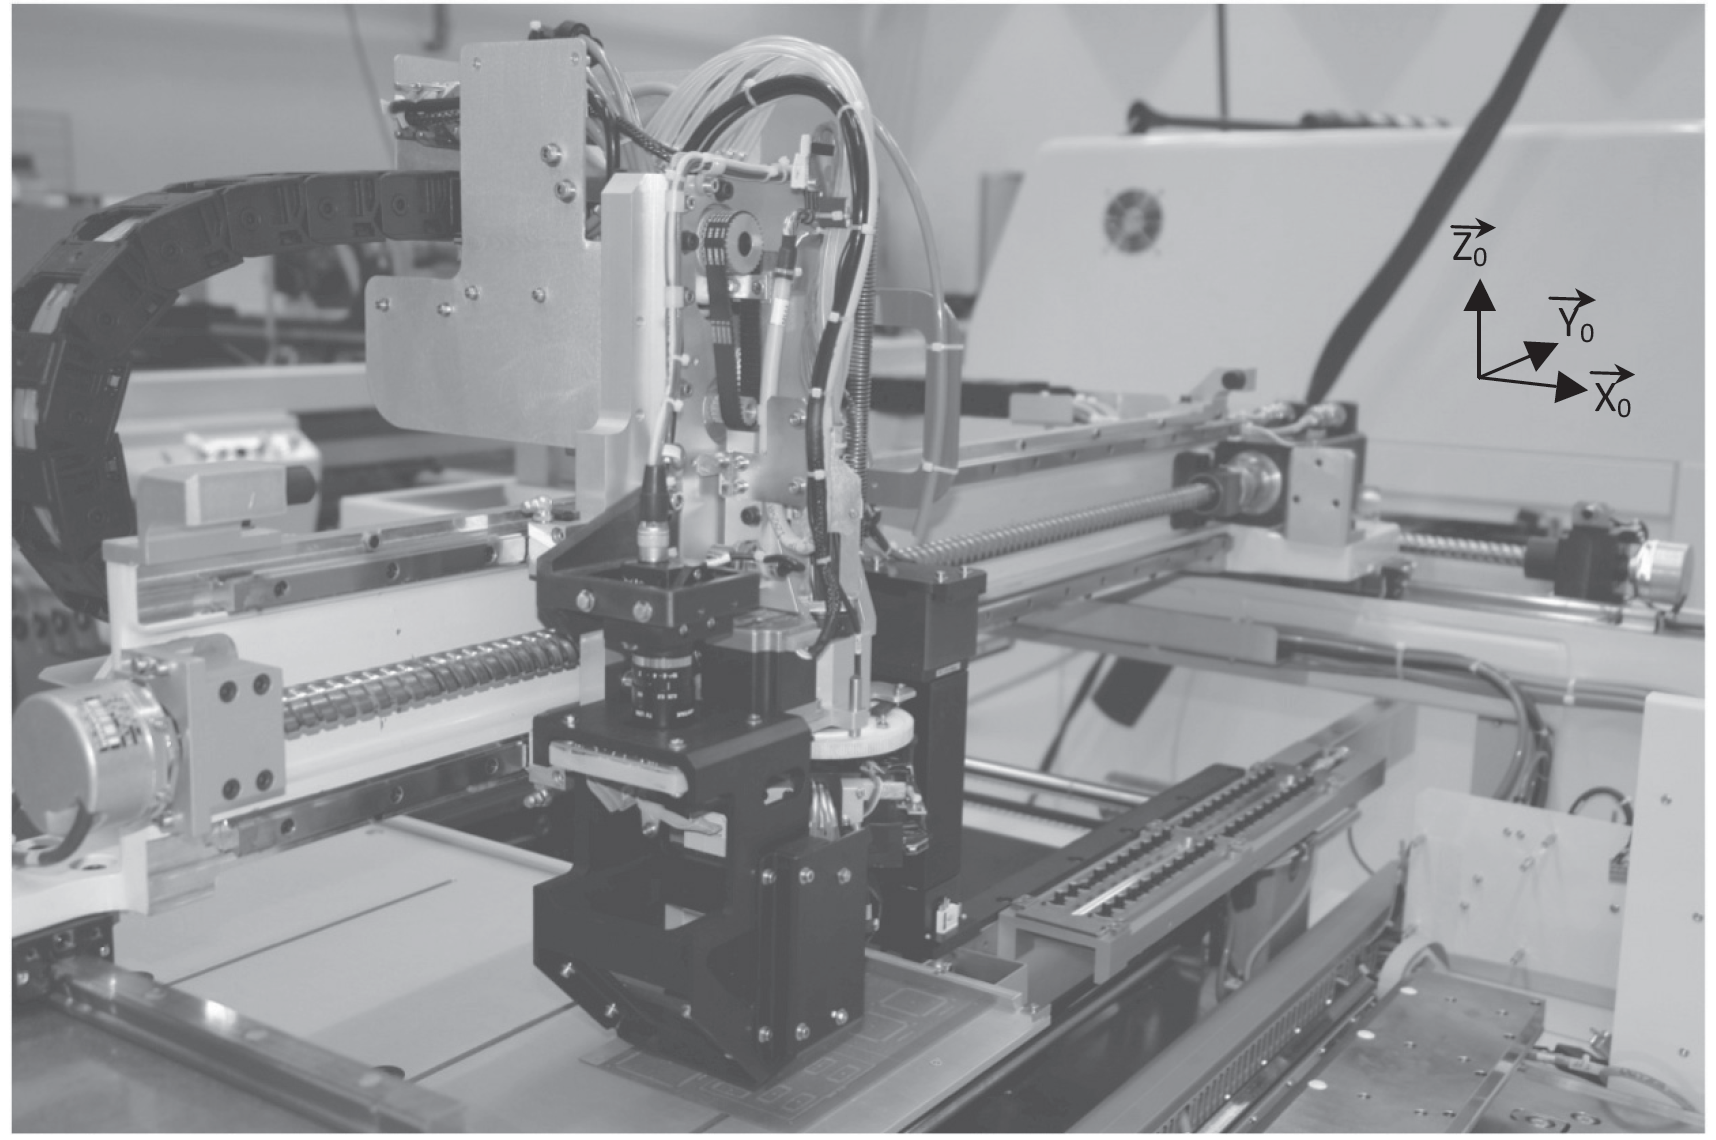
\includegraphics[width=.7\linewidth]{images/axe_y_photo}
}%figues de la page de garde


\iflivret
\pagestyle{empty}


%%%%%%%% PAGE DE GARDE COURS
\ifcours
% ==== BANDEAU DES TITRES ==== 
\begin{tikzpicture}[remember picture,overlay]
\node at (current page.north west)
{\begin{tikzpicture}[remember picture,overlay]
\node[anchor=north west,inner sep=0pt] at (0,0) {\includegraphics[width=\paperwidth]{\thechapterimage}};
\draw[anchor=west] (-2cm,-8cm) node [line width=2pt,rounded corners=15pt,draw=ocre,fill=white,fill opacity=0.6,inner sep=40pt]{\strut\makebox[22cm]{}};
\draw[anchor=west] (1cm,-8cm) node {\huge\sffamily\bfseries\color{black} %
\begin{minipage}{1cm}
\rotatebox{90}{\LARGE\sffamily\textsc{\color{ocre}\textbf{\xxnumpartie}}}
\end{minipage} \hfill
\begin{minipage}[c]{14cm}
\begin{titrepartie}
\begin{flushright}
\renewcommand{\baselinestretch}{1.1} 
\Large\sffamily\textsc{\textbf{\xxpartie}}
\renewcommand{\baselinestretch}{1} 
\end{flushright}
\end{titrepartie}
\end{minipage} \hfill
\begin{minipage}[c]{3.5cm}
{\large\sffamily\textsc{\textbf{\color{ocre} \discipline}}}
\end{minipage} 
 };
\end{tikzpicture}};
\end{tikzpicture}
% ==== FIN BANDEAU DES TITRES ==== 


% ==== ONGLET 
\begin{tikzpicture}[overlay]
\node[shape=rectangle, 
      rounded corners = .25 cm,
	  draw= ocre,
	  line width=2pt, 
	  fill = ocre!10,
	  minimum width  = 2.5cm,
	  minimum height = 3cm,] at (18.3cm,0) {};
\node at (17.7cm,0) {\rotatebox{90}{\textbf{\Large\color{ocre}{\classe}}}};
%{};
\end{tikzpicture}
% ==== FIN ONGLET 


\vspace{3.5cm}

\begin{tikzpicture}[remember picture,overlay]
\draw[anchor=west] (-2cm,-6cm) node {\huge\sffamily\bfseries\color{black} %
\begin{minipage}{2cm}
\begin{center}
\LARGE\sffamily\textsc{\color{ocre}\textbf{\xxactivite}}
\end{center}
\end{minipage} \hfill
\begin{minipage}[c]{15cm}
\begin{titrechapitre}
\renewcommand{\baselinestretch}{1.1} 
\Large\sffamily\textsc{\textbf{\xxnumchapitre}}

\Large\sffamily\textsc{\textbf{\xxchapitre}}
\vspace{.5cm}

\renewcommand{\baselinestretch}{1} 
\normalsize\normalfont
\xxcompetences
\end{titrechapitre}
\end{minipage}  };
\end{tikzpicture}
\vfill

\begin{flushright}
\begin{minipage}[c]{.3\linewidth}
\begin{center}
\xxfigures
\end{center}
\end{minipage}\hfill
\begin{minipage}[c]{.6\linewidth}
\startcontents
%\printcontents{}{1}{}
\printcontents{}{1}{}
\end{minipage}
\end{flushright}

\begin{tikzpicture}[remember picture,overlay]
\draw[anchor=west] (4.5cm,-.7cm) node {
\begin{minipage}[c]{.2\linewidth}
\begin{flushright}

\includegraphics[width=2cm]{logoCC}
\end{flushright}
\end{minipage}
\begin{minipage}[c]{.2\linewidth}
\textsl{\xxauteur} \\
\textsl{\classe}
\end{minipage}
 };
\end{tikzpicture}

\newpage
\pagestyle{fancy}

%\newpage
%\pagestyle{fancy}

\else
\fi
%% FIN PAGE DE GARDE DES COURS

%%%%%%%% PAGE DE GARDE TD
\iftd
%\begin{tikzpicture}[remember picture,overlay]
%\node at (current page.north west)
%{\begin{tikzpicture}[remember picture,overlay]
%\draw[anchor=west] (-2cm,-3.25cm) node [line width=2pt,rounded corners=15pt,draw=ocre,fill=white,fill opacity=0.6,inner sep=40pt]{\strut\makebox[22cm]{}};
%\draw[anchor=west] (1cm,-3.25cm) node {\huge\sffamily\bfseries\color{black} %
%\begin{minipage}{1cm}
%\rotatebox{90}{\LARGE\sffamily\textsc{\color{ocre}\textbf{\xxnumpartie}}}
%\end{minipage} \hfill
%\begin{minipage}[c]{13.5cm}
%\begin{titrepartie}
%\begin{flushright}
%\renewcommand{\baselinestretch}{1.1} 
%\Large\sffamily\textsc{\textbf{\xxpartie}}
%\renewcommand{\baselinestretch}{1} 
%\end{flushright}
%\end{titrepartie}
%\end{minipage} \hfill
%\begin{minipage}[c]{3.5cm}
%{\large\sffamily\textsc{\textbf{\color{ocre} \discipline}}}
%\end{minipage} 
% };
%\end{tikzpicture}};
%\end{tikzpicture}

%%%%%%%%%% PAGE DE GARDE TD %%%%%%%%%%%%%%%
%\begin{tikzpicture}[overlay]
%\node[shape=rectangle, 
%      rounded corners = .25 cm,
%	  draw= ocre,
%	  line width=2pt, 
%	  fill = ocre!10,
%	  minimum width  = 2.5cm,
%	  minimum height = 2.5cm,] at (18.5cm,0) {};
%\node at (17.7cm,0) {\rotatebox{90}{\textbf{\Large\color{ocre}{\classe}}}};
%%{};
%\end{tikzpicture}

% PARTIE ET CHAPITRE
%\begin{tikzpicture}[remember picture,overlay]
%\draw[anchor=west] (-1cm,-2.1cm) node {\large\sffamily\bfseries\color{black} %
%\begin{minipage}[c]{15cm}
%\begin{flushleft}
%\xxnumchapitre \\
%\xxchapitre
%\end{flushleft}
%\end{minipage}  };
%\end{tikzpicture}

% BANDEAU EXO
\iflivret % SI LIVRET
\begin{tikzpicture}[remember picture,overlay]
\draw[anchor=west] (-2cm,-3.3cm) node {\huge\sffamily\bfseries\color{black} %
\begin{minipage}{5cm}
\begin{center}
\LARGE\sffamily\color{ocre}\textbf{\textsc{\xxactivite}}

\begin{center}
\xxfigures
\end{center}

\end{center}
\end{minipage} \hfill
\begin{minipage}[c]{12cm}
\begin{titrechapitre}
\renewcommand{\baselinestretch}{1.1} 
\large\sffamily\textbf{\textsc{\xxtitreexo}}

\small\sffamily{\textbf{\textit{\color{black!70}\xxsourceexo}}}
\vspace{.5cm}

\renewcommand{\baselinestretch}{1} 
\normalsize\normalfont
\xxcompetences
\end{titrechapitre}
\end{minipage}};
\end{tikzpicture}
\else % ELSE NOT LIVRET
\begin{tikzpicture}[remember picture,overlay]
\draw[anchor=west] (-2cm,-4.5cm) node {\huge\sffamily\bfseries\color{black} %
\begin{minipage}{5cm}
\begin{center}
\LARGE\sffamily\color{ocre}\textbf{\textsc{\xxactivite}}

\begin{center}
\xxfigures
\end{center}

\end{center}
\end{minipage} \hfill
\begin{minipage}[c]{12cm}
\begin{titrechapitre}
\renewcommand{\baselinestretch}{1.1} 
\large\sffamily\textbf{\textsc{\xxtitreexo}}

\small\sffamily{\textbf{\textit{\color{black!70}\xxsourceexo}}}
\vspace{.5cm}

\renewcommand{\baselinestretch}{1} 
\normalsize\normalfont
\xxcompetences
\end{titrechapitre}
\end{minipage}};
\end{tikzpicture}

\fi

\else   % FIN IF TD
\fi


%%%%%%%% PAGE DE GARDE FICHE
\iffiche
\begin{tikzpicture}[remember picture,overlay]
\node at (current page.north west)
{\begin{tikzpicture}[remember picture,overlay]
\draw[anchor=west] (-2cm,-2.25cm) node [line width=2pt,rounded corners=15pt,draw=ocre,fill=white,fill opacity=0.6,inner sep=40pt]{\strut\makebox[22cm]{}};
\draw[anchor=west] (1cm,-2.25cm) node {\huge\sffamily\bfseries\color{black} %
\begin{minipage}{1cm}
\rotatebox{90}{\LARGE\sffamily\textsc{\color{ocre}\textbf{\xxnumpartie}}}
\end{minipage} \hfill
\begin{minipage}[c]{14cm}
\begin{titrepartie}
\begin{flushright}
\renewcommand{\baselinestretch}{1.1} 
\large\sffamily\textsc{\textbf{\xxpartie} \\} 

\vspace{.2cm}

\normalsize\sffamily\textsc{\textbf{\xxnumchapitre -- \xxchapitre}}
\renewcommand{\baselinestretch}{1} 
\end{flushright}
\end{titrepartie}
\end{minipage} \hfill
\begin{minipage}[c]{3.5cm}
{\large\sffamily\textsc{\textbf{\color{ocre} \discipline}}}
\end{minipage} 
 };
\end{tikzpicture}};
\end{tikzpicture}

\iflivret
\begin{tikzpicture}[overlay]
\node[shape=rectangle, 
      rounded corners = .25 cm,
	  draw= ocre,
	  line width=2pt, 
	  fill = ocre!10,
	  minimum width  = 2.5cm,
	  minimum height = 2.5cm,] at (18.5cm,.5cm) {};
\node at (17.9cm,.5cm) {\rotatebox{90}{\textsf{\textbf{\large\color{ocre}{\classe}}}}};
%{};
\end{tikzpicture}
\else
\begin{tikzpicture}[overlay]
\node[shape=rectangle, 
      rounded corners = .25 cm,
	  draw= ocre,
	  line width=2pt, 
	  fill = ocre!10,
	  minimum width  = 2.5cm,
%	  minimum height = 2.5cm,] at (18.5cm,1.1cm) {};
	  minimum height = 2.5cm,] at (18.6cm,0.5cm) {};
\node at (18cm,0.5cm) {\rotatebox{90}{\textsf{\textbf{\large\color{ocre}{\classe}}}}};
%{};
\end{tikzpicture}

\fi

\else
\fi



\else
\pagestyle{empty}


%%%%%%%% PAGE DE GARDE COURS
\ifcours
% ==== BANDEAU DES TITRES ==== 
\begin{tikzpicture}[remember picture,overlay]
\node at (current page.north west)
{\begin{tikzpicture}[remember picture,overlay]
\node[anchor=north west,inner sep=0pt] at (0,0) {\includegraphics[width=\paperwidth]{\thechapterimage}};
\draw[anchor=west] (-2cm,-8cm) node [line width=2pt,rounded corners=15pt,draw=ocre,fill=white,fill opacity=0.6,inner sep=40pt]{\strut\makebox[22cm]{}};
\draw[anchor=west] (1cm,-8cm) node {\huge\sffamily\bfseries\color{black} %
\begin{minipage}{1cm}
\rotatebox{90}{\LARGE\sffamily\textsc{\color{ocre}\textbf{\xxnumpartie}}}
\end{minipage} \hfill
\begin{minipage}[c]{14cm}
\begin{titrepartie}
\begin{flushright}
\renewcommand{\baselinestretch}{1.1} 
\Large\sffamily\textsc{\textbf{\xxpartie}}
\renewcommand{\baselinestretch}{1} 
\end{flushright}
\end{titrepartie}
\end{minipage} \hfill
\begin{minipage}[c]{3.5cm}
{\large\sffamily\textsc{\textbf{\color{ocre} \discipline}}}
\end{minipage} 
 };
\end{tikzpicture}};
\end{tikzpicture}
% ==== FIN BANDEAU DES TITRES ==== 


% ==== ONGLET 
\begin{tikzpicture}[overlay]
\node[shape=rectangle, 
      rounded corners = .25 cm,
	  draw= ocre,
	  line width=2pt, 
	  fill = ocre!10,
	  minimum width  = 2.5cm,
	  minimum height = 3cm,] at (18.3cm,0) {};
\node at (17.7cm,0) {\rotatebox{90}{\textbf{\Large\color{ocre}{\classe}}}};
%{};
\end{tikzpicture}
% ==== FIN ONGLET 


\vspace{3.5cm}

\begin{tikzpicture}[remember picture,overlay]
\draw[anchor=west] (-2cm,-6cm) node {\huge\sffamily\bfseries\color{black} %
\begin{minipage}{2cm}
\begin{center}
\LARGE\sffamily\textsc{\color{ocre}\textbf{\xxactivite}}
\end{center}
\end{minipage} \hfill
\begin{minipage}[c]{15cm}
\begin{titrechapitre}
\renewcommand{\baselinestretch}{1.1} 
\Large\sffamily\textsc{\textbf{\xxnumchapitre}}

\Large\sffamily\textsc{\textbf{\xxchapitre}}
\vspace{.5cm}

\renewcommand{\baselinestretch}{1} 
\normalsize\normalfont
\xxcompetences
\end{titrechapitre}
\end{minipage}  };
\end{tikzpicture}
\vfill

\begin{flushright}
\begin{minipage}[c]{.3\linewidth}
\begin{center}
\xxfigures
\end{center}
\end{minipage}\hfill
\begin{minipage}[c]{.6\linewidth}
\startcontents
%\printcontents{}{1}{}
\printcontents{}{1}{}
\end{minipage}
\end{flushright}

\begin{tikzpicture}[remember picture,overlay]
\draw[anchor=west] (4.5cm,-.7cm) node {
\begin{minipage}[c]{.2\linewidth}
\begin{flushright}

\includegraphics[width=2cm]{logoCC}
\end{flushright}
\end{minipage}
\begin{minipage}[c]{.2\linewidth}
\textsl{\xxauteur} \\
\textsl{\classe}
\end{minipage}
 };
\end{tikzpicture}

\newpage
\pagestyle{fancy}

%\newpage
%\pagestyle{fancy}

\else
\fi
%% FIN PAGE DE GARDE DES COURS

%%%%%%%% PAGE DE GARDE TD
\iftd
%\begin{tikzpicture}[remember picture,overlay]
%\node at (current page.north west)
%{\begin{tikzpicture}[remember picture,overlay]
%\draw[anchor=west] (-2cm,-3.25cm) node [line width=2pt,rounded corners=15pt,draw=ocre,fill=white,fill opacity=0.6,inner sep=40pt]{\strut\makebox[22cm]{}};
%\draw[anchor=west] (1cm,-3.25cm) node {\huge\sffamily\bfseries\color{black} %
%\begin{minipage}{1cm}
%\rotatebox{90}{\LARGE\sffamily\textsc{\color{ocre}\textbf{\xxnumpartie}}}
%\end{minipage} \hfill
%\begin{minipage}[c]{13.5cm}
%\begin{titrepartie}
%\begin{flushright}
%\renewcommand{\baselinestretch}{1.1} 
%\Large\sffamily\textsc{\textbf{\xxpartie}}
%\renewcommand{\baselinestretch}{1} 
%\end{flushright}
%\end{titrepartie}
%\end{minipage} \hfill
%\begin{minipage}[c]{3.5cm}
%{\large\sffamily\textsc{\textbf{\color{ocre} \discipline}}}
%\end{minipage} 
% };
%\end{tikzpicture}};
%\end{tikzpicture}

%%%%%%%%%% PAGE DE GARDE TD %%%%%%%%%%%%%%%
%\begin{tikzpicture}[overlay]
%\node[shape=rectangle, 
%      rounded corners = .25 cm,
%	  draw= ocre,
%	  line width=2pt, 
%	  fill = ocre!10,
%	  minimum width  = 2.5cm,
%	  minimum height = 2.5cm,] at (18.5cm,0) {};
%\node at (17.7cm,0) {\rotatebox{90}{\textbf{\Large\color{ocre}{\classe}}}};
%%{};
%\end{tikzpicture}

% PARTIE ET CHAPITRE
%\begin{tikzpicture}[remember picture,overlay]
%\draw[anchor=west] (-1cm,-2.1cm) node {\large\sffamily\bfseries\color{black} %
%\begin{minipage}[c]{15cm}
%\begin{flushleft}
%\xxnumchapitre \\
%\xxchapitre
%\end{flushleft}
%\end{minipage}  };
%\end{tikzpicture}

% BANDEAU EXO
\iflivret % SI LIVRET
\begin{tikzpicture}[remember picture,overlay]
\draw[anchor=west] (-2cm,-3.3cm) node {\huge\sffamily\bfseries\color{black} %
\begin{minipage}{5cm}
\begin{center}
\LARGE\sffamily\color{ocre}\textbf{\textsc{\xxactivite}}

\begin{center}
\xxfigures
\end{center}

\end{center}
\end{minipage} \hfill
\begin{minipage}[c]{12cm}
\begin{titrechapitre}
\renewcommand{\baselinestretch}{1.1} 
\large\sffamily\textbf{\textsc{\xxtitreexo}}

\small\sffamily{\textbf{\textit{\color{black!70}\xxsourceexo}}}
\vspace{.5cm}

\renewcommand{\baselinestretch}{1} 
\normalsize\normalfont
\xxcompetences
\end{titrechapitre}
\end{minipage}};
\end{tikzpicture}
\else % ELSE NOT LIVRET
\begin{tikzpicture}[remember picture,overlay]
\draw[anchor=west] (-2cm,-4.5cm) node {\huge\sffamily\bfseries\color{black} %
\begin{minipage}{5cm}
\begin{center}
\LARGE\sffamily\color{ocre}\textbf{\textsc{\xxactivite}}

\begin{center}
\xxfigures
\end{center}

\end{center}
\end{minipage} \hfill
\begin{minipage}[c]{12cm}
\begin{titrechapitre}
\renewcommand{\baselinestretch}{1.1} 
\large\sffamily\textbf{\textsc{\xxtitreexo}}

\small\sffamily{\textbf{\textit{\color{black!70}\xxsourceexo}}}
\vspace{.5cm}

\renewcommand{\baselinestretch}{1} 
\normalsize\normalfont
\xxcompetences
\end{titrechapitre}
\end{minipage}};
\end{tikzpicture}

\fi

\else   % FIN IF TD
\fi


%%%%%%%% PAGE DE GARDE FICHE
\iffiche
\begin{tikzpicture}[remember picture,overlay]
\node at (current page.north west)
{\begin{tikzpicture}[remember picture,overlay]
\draw[anchor=west] (-2cm,-2.25cm) node [line width=2pt,rounded corners=15pt,draw=ocre,fill=white,fill opacity=0.6,inner sep=40pt]{\strut\makebox[22cm]{}};
\draw[anchor=west] (1cm,-2.25cm) node {\huge\sffamily\bfseries\color{black} %
\begin{minipage}{1cm}
\rotatebox{90}{\LARGE\sffamily\textsc{\color{ocre}\textbf{\xxnumpartie}}}
\end{minipage} \hfill
\begin{minipage}[c]{14cm}
\begin{titrepartie}
\begin{flushright}
\renewcommand{\baselinestretch}{1.1} 
\large\sffamily\textsc{\textbf{\xxpartie} \\} 

\vspace{.2cm}

\normalsize\sffamily\textsc{\textbf{\xxnumchapitre -- \xxchapitre}}
\renewcommand{\baselinestretch}{1} 
\end{flushright}
\end{titrepartie}
\end{minipage} \hfill
\begin{minipage}[c]{3.5cm}
{\large\sffamily\textsc{\textbf{\color{ocre} \discipline}}}
\end{minipage} 
 };
\end{tikzpicture}};
\end{tikzpicture}

\iflivret
\begin{tikzpicture}[overlay]
\node[shape=rectangle, 
      rounded corners = .25 cm,
	  draw= ocre,
	  line width=2pt, 
	  fill = ocre!10,
	  minimum width  = 2.5cm,
	  minimum height = 2.5cm,] at (18.5cm,.5cm) {};
\node at (17.9cm,.5cm) {\rotatebox{90}{\textsf{\textbf{\large\color{ocre}{\classe}}}}};
%{};
\end{tikzpicture}
\else
\begin{tikzpicture}[overlay]
\node[shape=rectangle, 
      rounded corners = .25 cm,
	  draw= ocre,
	  line width=2pt, 
	  fill = ocre!10,
	  minimum width  = 2.5cm,
%	  minimum height = 2.5cm,] at (18.5cm,1.1cm) {};
	  minimum height = 2.5cm,] at (18.6cm,0.5cm) {};
\node at (18cm,0.5cm) {\rotatebox{90}{\textsf{\textbf{\large\color{ocre}{\classe}}}}};
%{};
\end{tikzpicture}

\fi

\else
\fi



\fi
\setlength{\columnseprule}{.1pt}

\pagestyle{fancy}
\thispagestyle{plain}

\ifprof
\vspace{5.1cm}
\else
\vspace{4.9cm}
\fi

\def\columnseprulecolor{\color{ocre}}
\setlength{\columnseprule}{0.4pt} 

%%%%%%%%%%%%%%%%%%%%%%%

\setcounter{exo}{0}



\ifprof
%\begin{multicols}{2}
\else
\begin{multicols}{2}
\fi


\section*{Présentation du système}
\ifprof
\else
Le système étudié permet de déposer automatiquement des composants électroniques sur un circuit.
On s'intéresse ici à la modélisation d'un seul axe (selon la direction notée $\overrightarrow{y_0}$). actionné par un moteur électrique et utilisant un mécanisme de transformation de mouvement.
%
%On donne les exigences associées au système : 
%
%\begin{center}
%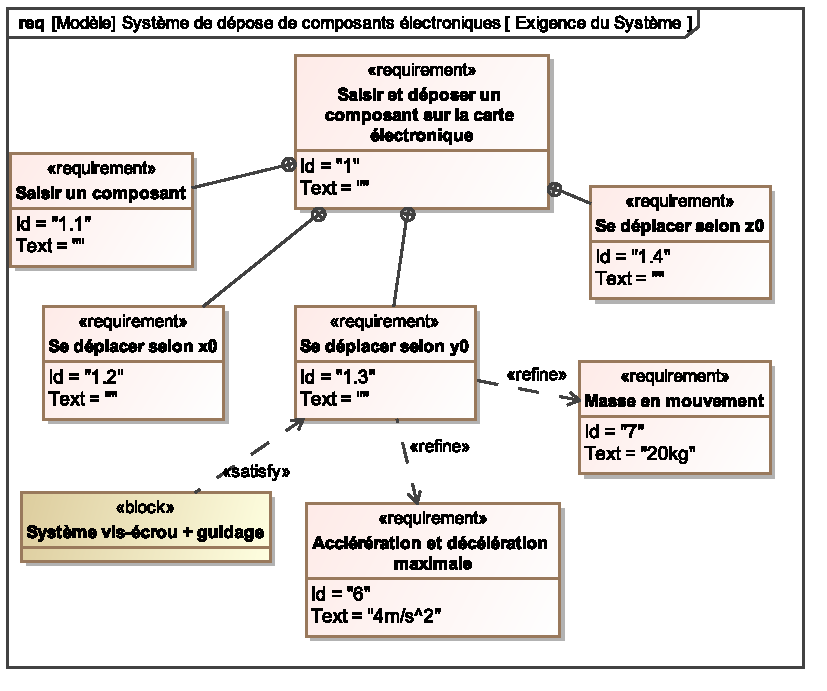
\includegraphics[width=\linewidth]{images/req_systeme_depose.pdf}
%\end{center}


\textbf{Hypothèses :}
\begin{itemize}
\item le référentiel associé au repère $R_0=\quadruplet{O_0}{\overrightarrow{x_0}}{\overrightarrow{y_0}}{\overrightarrow{z_0}}$ est supposé galiléen ;
\item les solides seront supposés indéformables ; 
\item on notera $J_1$ le moment d'inertie du solide 1 selon l'axe $\couple{O_0}{y_0}$ : $J_1=I_{\couple{O_0}{y_0}}(S_1)$ ;
\item on note $M_3$ et $G_3$ respectivement la masse et le centre d'inertie du solide $S_3$ ;
\item la position de $G_3$ est définie par $\overrightarrow{O_0G_3}=x\overrightarrow{x_0}+y \overrightarrow{y_0}+z \overrightarrow{z_0}$
\item les liaisons sont supposées parfaites (sans jeu ni frottement).
\end{itemize}

Le système est modélisé par le schéma cinématique ci-dessous :
\begin{center}
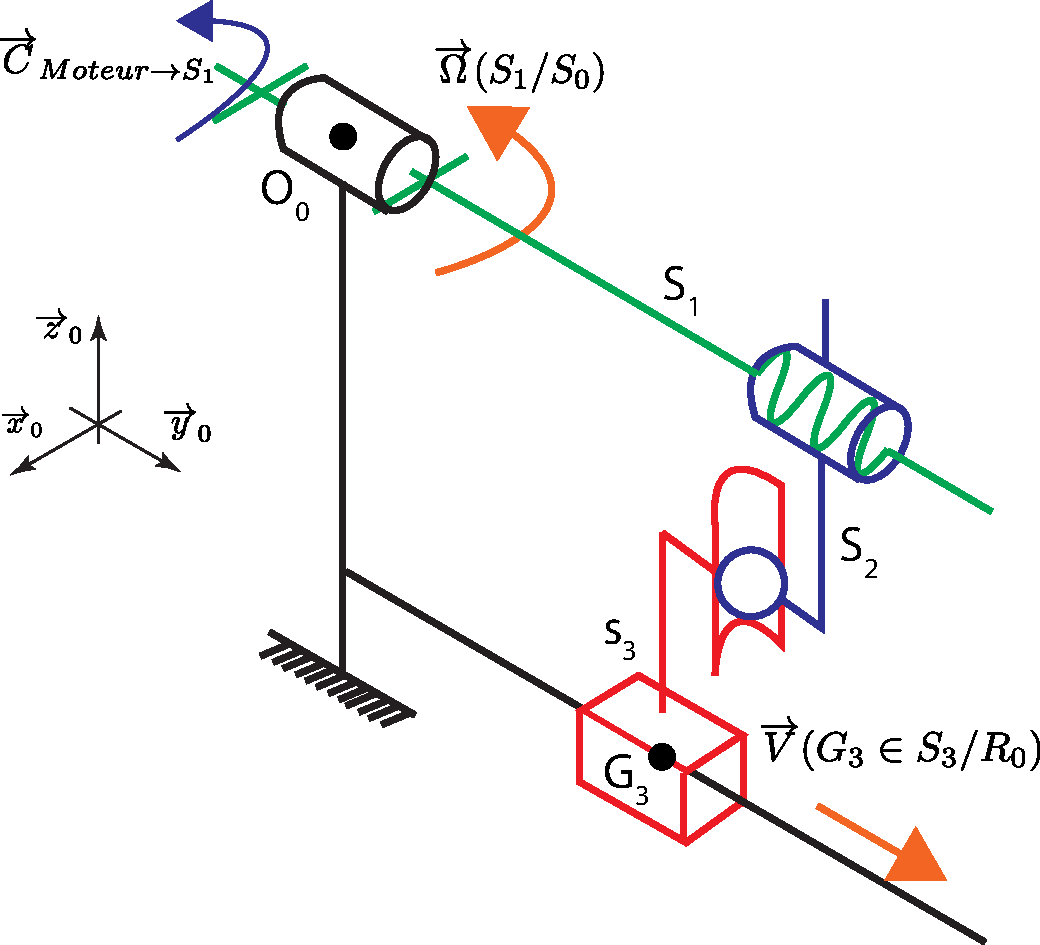
\includegraphics[width=0.6\linewidth]{images/schema_cine_depose_composant.pdf}
\end{center}

On note : 
\begin{itemize}
\item $S_0$ : poutre transversale considérée comme fixe par rapport au bâti ;
\item $S_1$ : vis à billes (hélice à droite) de pas $p=\SI{20}{mm}$;
\item $S_2$ : écrou de la vis à billes ;
\item $S_3$ : chariot supportant la tête de dépose (masse $M_3$).
\end{itemize}


On donne les caractéristiques du moteur entraînant l'axe et la vis $S_1$ :
\begin{itemize}
%\item couple maximal, $C_{\text{max}} = \SI{21,2}{N.m}$ ;
%\item fréquence de rotation maximale, $N_m = \SI{6000}{tr/min}$;
\item moment d'inertie du moteur suivant l'axe $\overrightarrow{y_0}$ : $I_m = \SI{1,6}{10^{-4} kg.m^2}$ ;
\item moment d'inertie de la vis à billes suivant l'axe $\overrightarrow{y_0}$ : $I_v = 2,1\,  10^{-4}\text{kg m}^2$.
\end{itemize}
De plus $\overrightarrow{\Omega}(S_1/R_0)=\dot{\theta}(t)\cdot \overrightarrow{y_0}$

\fi
\begin{obj}
L'objectif de cette étude est de relier les grandeurs liées à l'actionneur du système (moteur) :
\begin{itemize}
\item couple transmis à $S_1$ : $\overrightarrow{C}_{\text{Moteur}\to S_1}$ ;
\item vitesse de rotation de $S_1$ : $\overrightarrow{\Omega}(S_1/R_0)\cdot \overrightarrow{y}_0=\dot{\theta}$.
\end{itemize} 
à celles liée à l'effecteur (tête de dépose $S_3$) : 
\begin{itemize}
\item masse : $M_3$;
\item cinématique de $S_3$ : $\vectg{G_3}{S_3}{R_0}\cdot \overrightarrow{y}_0=\ddot{y}$.
\end{itemize}
\end{obj}



%\begin{exemple}[Machine de dépose de composants électroniques : déplacement dynamique de $S_3$]
%\begin{minipage}{0.35\textwidth}


\subparagraph{}
\textit{Réaliser le graphe de structure associé au mécanisme.}

\subparagraph{}
\textit{Proposer une stratégie pour répondre à l'objectif.}

\subparagraph{}
\textit{Déterminer la relation entre l'effort de poussée dans la liaison linéaire annulaire et l'accélération du chariot.}
\ifprof
\begin{corrige}
On connaît la masse $M_3$ de la tête de dépose et on cherche l'effort ($\overrightarrow{R}_{\text{poussée}\to S_3}$) de poussée que doit fournir l'actionneur pour obtenir l'accélération souhaitée.

\begin{center}
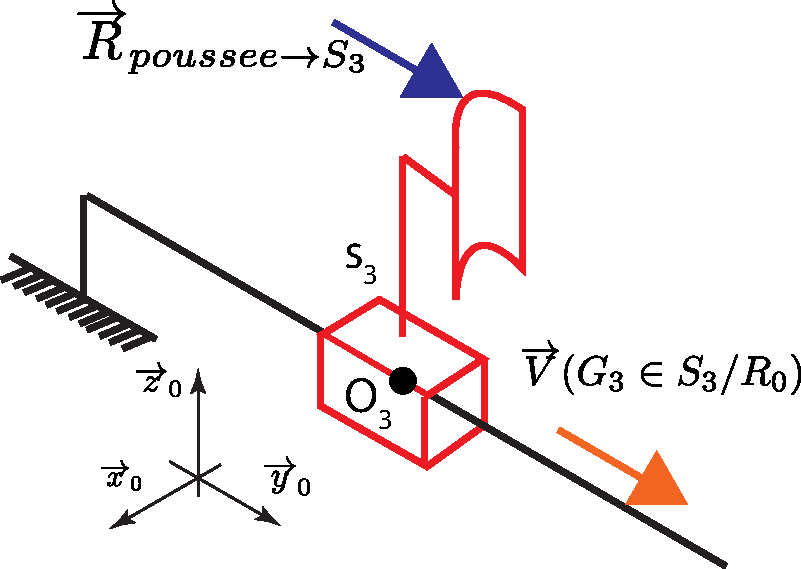
\includegraphics[width=.4\linewidth]{images/schema_cine_depose_translation.pdf}
\end{center}
%\end{minipage}

On utilise le théorème de la résultante dynamique en projection sur $\overrightarrow{y_0}$. On obtient : $
M_3 \vectg{G_3}{3}{R_0}\cdot \overrightarrow{y_0}=\sum \overrightarrow{R}_{\text{ext}\to S_3}\cdot \overrightarrow{y_0}$.
 
%Au final $M_3\cdot \ddot{y}=R_{\text{pouss\'ee}\to S_3}$.
Au final $M_3\cdot \ddot{y}=Y_{23}$.


\textit{Application numérique : } détermination de $R_{\text{pouss\'ee}\to S_3}$ pour obtenir une accélération de $\SI{4}{m/s^2}$ : $R_{\text{pouss\'ee}\to S_3}=20\times 4=\SI{80}{N}
$.
\end{corrige}
%\end{texteCache}
%\end{exemple}
\else
\fi


\subparagraph{}
\textit{Déterminer la relation entre le couple moteur et le couple transmis dans la liaison hélicoïdale.}


\ifprof
\begin{corrige}
%\begin{exemple}[Machine de dépose de composants électroniques : déplacement dynamique de $S_3$]
%\begin{minipage}{0.5\textwidth}
%\end{minipage}
%\begin{minipage}{0.45\textwidth}
\begin{center}
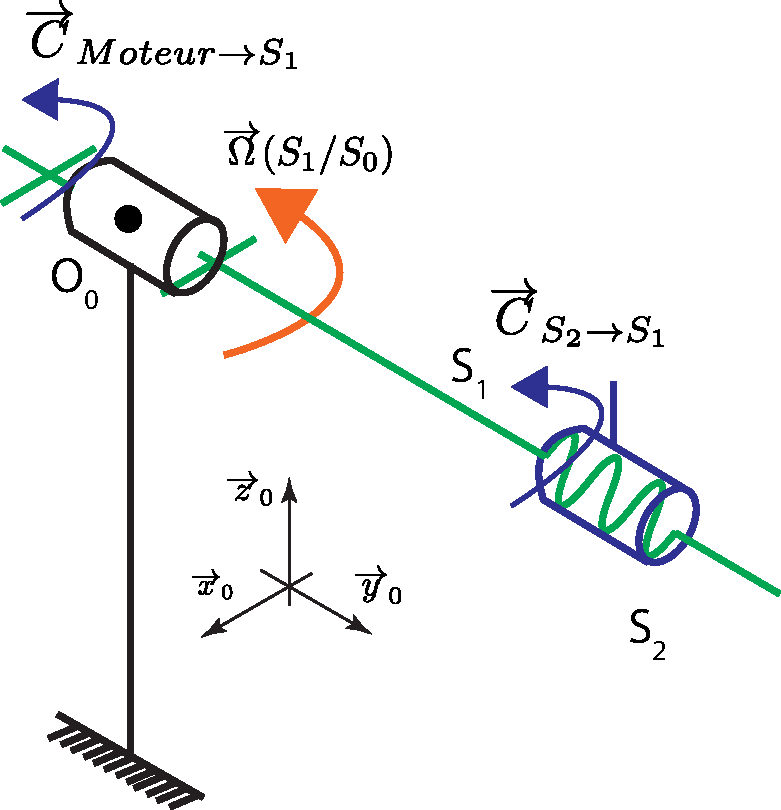
\includegraphics[width=.4\linewidth]{images/schema_cine_depose_rotation.pdf}
\end{center}
%\end{minipage}

\textbf{Détermination des caractéristiques maximales : }


On se place de la cas le plus limite (Couple maximal, accélération angulaire constante pour atteindre la fréquence de rotation maximale en $t_a=\SI{0,2}{s}$)
Déterminer le couple résistant maximal que le moteur peut équilibrer dynamiquement ($C_{S_2\to S_1}$):

%\begin{texteCache}
En appliquant un théorème du moment dynamique à $S_1$ selon $\couple{O_0}{{y}_0}$ :
$(I_m+I_v)\cdot \ddot{\theta}=C_{\text{max}}+C_{S_2\to S_1}$. 

On obtient alors : 
$C_{S_2\to S_1}=(I_m+I_v)\cdot \ddot{\theta}_{\text{max}}-C_{\text{max}}=(I_m+I_v)\cdot \frac{N_m\times 2\cdot \pi}{60\cdot t_a}-C_{\text{max}}=-\SI{20}{Nm}$.

%\end{texteCache}
%\end{exemple}


%\begin{bilan}
%\begin{itemize}
%\item Les deux cas présentés ci-dessus sont traités de manière indépendante.
%\item Le lien entre ces deux parties (actionneur et effecteur) repose sur le mécanisme de transformation de mouvement (ici vis-écrou).
%\item Il faudra donc procéder à une démarche de résolution globale pour relier le couple moteur $\overrightarrow{C}_{\text{moteur}\to S_1}$ à l'accélération ($\vectg{G_3}{3}{R_0}$) et la masse de l'effecteur ($M_3$). Ce sera l'objet des parties suivantes.
%\end{itemize}
\end{corrige}
\else
\fi


\subparagraph{}
\textit{Donner la relation entre le couple transmis par la liaison hélicoïdale et l'effort axial.}
\ifprof
\begin{corrige}
On a : $M_{12}=Y_{12}\dfrac{\text{pas}}{2\pi}$.
\end{corrige}
\else
\fi
\subparagraph{}
\textit{Déterminer la relation entre l'effort axial dans la liaison hélicoïdale et l'effort de poussée dans la liaison sphère -- cylindre.}
\ifprof
\begin{corrige}
On isole $S_2$, soumis aux actions mécaniques de $S_3$ et $S_1$. La masse de $S_2$ est négligée. 
On applique le TRD suivant $\vect{y_0}$ et on a : 
$$
Y_{32}+Y_{12}=0 \Leftrightarrow 
Y_{23}=Y_{12}
$$
\end{corrige}
\else
\fi


\subparagraph{}
\textit{Quel doit être le couple moteur pour déplacer le chariot $S_3$ ?}
\ifprof
\begin{corrige}
On a : 
\begin{itemize}
\item $M_{12}=Y_{12}\dfrac{\text{pas}}{2\pi} \Leftrightarrow M_{21}=-Y_{12}\dfrac{\text{pas}}{2\pi}$;
\item $Y_{23}=Y_{12}$;
\item $(I_m+I_v)\cdot \ddot{\theta}=C_{\text{max}}+M_{21}$;
\item $M_3\cdot \ddot{y}=Y_{23}$.
\end{itemize}

On a donc $C_{\text{max}}=(I_m+I_v)\cdot \ddot{\theta}+M_3 \ddot{y}\dfrac{\text{pas}}{2\pi}$
\end{corrige}
\else
\fi

Le cahier des charges impose les performances dynamiques suivantes : 
\begin{itemize}
\item l'accélération minimale de l'axe transversal est de \SI{21}{m.s^{-2}};
\item la vitesse minimale pour respecter la cadence souhaitée est de \SI{7}{m.s^{-1}};
\item la course de l'axe est de \SI{2}{m}.
\end{itemize}

La loi de commande est une loi en trapèze de vitesse. 
\subparagraph{}
\textit{Donner les caractéristiques dynamiques que doit respecter le moteur.}
\ifprof
\begin{corrige}
Avec un pas de \SI{20}{mm}, $\dot{\theta}=\dot{y}\dfrac{2\pi}{\text{pas}}$ et $\ddot{\theta}=\ddot{y}\dfrac{2\pi}{\text{pas}}$. 

AN : $\dot{\theta}=7\cdot 2\pi/20 10^3=\SI{2200}{rad.s^{-1}}=\SI{230}{tr.min^{-1}}$ et $\ddot{\theta}=21\cdot 2\pi/20 10^3 = \SI{6600}{rad.s^{-2}}$.
\end{corrige}
\else
\fi

\subparagraph{}
\textit{Quel est le temps nécessaire pour parcourir la course de la machine ? Commenter.}
\ifprof
\begin{corrige}
\begin{itemize}
\item Temps d'accélération pour atteindre la vitesse maximale : $V_m = a_m T_a \Leftrightarrow T_a = \dfrac{V_m}{a_m}=\SI{0,33}{s}$. 
%\item Distance totale : $2=2\dfrac{1}{2}T_aV_m + T_mV_m \Longleftrightarrow T_m = \dfrac{2-T_aV_m}{V_m}=$.
\item Distance parcourue : $\dfrac{1}{2}T_aV_m = \SI{1,17}{m}$. 
\end{itemize}
En conséquence, la course de la machine ne permet pas d'atteindre la vitesse maximale. 

Temps pour parcourir $\SI{1}{m}$ : $\dfrac{1}{2}a_mT_a^2 =1 \Rightarrow T_a = \dfrac{2}{21}=\SI{0,309}{s}$. Temps pour parcourir la course : \SI{0,62}{m}.
\end{corrige}
\else
\fi

%\subparagraph{}
%\textit{Quelle est la distance minimale à parcourir pour atteindre la vitesse maximale ?}
%\ifprof
%\begin{corrige}
%\end{corrige}
%\else
%\fi

\subparagraph{}
\textit{Quel est le couple que doit fournir le moteur pour déplacer le chariot dans le << pire des cas >> ?}
\ifprof
\begin{corrige}
\end{corrige}
\else
\fi



\ifprof
%\end{multicols}
\else
\end{multicols}
\fi

%\end{document}